\documentclass[12pt,a4paper]{scrartcl}
\usepackage[utf8]{inputenc}
\usepackage{amsmath}
\usepackage{amsfonts}
\usepackage{amssymb}
\usepackage{graphicx}
\usepackage[english, russian]{babel}

\title{}
\date{Егерев Артем, БПМИ-167}
\author{Домашняя работа по дискретной математике 15}

\begin{document}

\maketitle
\noindent Вспомогательные теормемы:\\
\textbf{1:} $\mathbb{Q}^n$ , где $n$ конечно  или счетно - счетно\\ 
\textbf{2:} $\mathbb{R} \sim \mathbb{R}^n \sim (0, 1) \sim [0, 1] \sim 2^{\mathbb{N}}$, где $n$ конечно или счетно, имеет мощность континум
\\ \\ \\

\noindent \textbf{Задача 1.} 
\textit{Да, верно.}  \\
\textit{Решение:} \\ 
Центр каждого круга есть пара чисел из $\mathbb{R}^2$ , радиус - число из $\mathbb{R}_+$. Каждый круг однозначно задается тройкой чисел: пара его координат  и радиус. Отсюда множество всех кругов на плоскости $\mathbb{R}_+ \mathbb{R}^2 \sim \mathbb{R}^3 \sim \mathbb{R}$ -  континум (Теорема 2).  
\\ \\ \\

\noindent \textbf{Задача 2.} \textit{Нет, неверно.} \\
\textit{Решение:} \\
Множество центров концентрических окружностей имеет мощность 1, в то время как их количество $\mathbb{R}_+$ - равномощно континому (количество всевозможных радиусов).
\\ \\ \\


\noindent \textbf{Задача 3.} \textit{Да, существует.}\\
\textit{Решение:} \\ 
Наглядно: \\
\begin{center}
	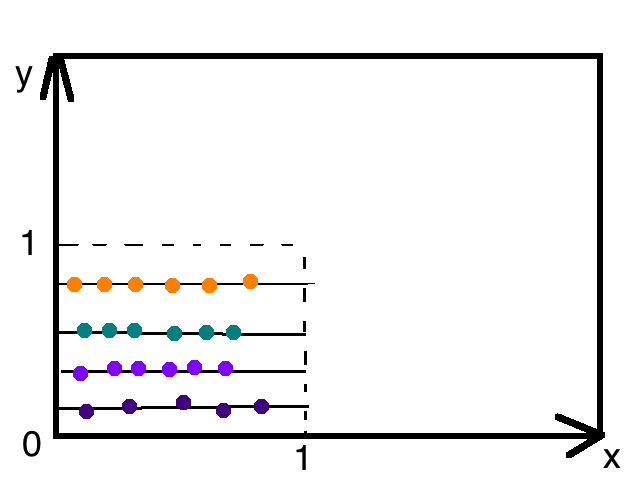
\includegraphics[height = 100pt]{3.png}	
\end{center}
Здесь множество линий (множество континуальных семейств) из $y$  - определено на [0, 1] - имеет мощность континум (Теорема 2). Каждая линия (отрезок)   есть интервал [0, 1] - так же   имеет континум точек. Все точки есть подмножество $\mathbb{R}^2$, из которого есть неявная биекция в $\mathbb{R} \Rightarrow$ континуальное множество континуальных подмножеств $\mathbb{R}$ существует.
\\ \\ \\


\noindent \textbf{Задача 4.} 
\textit{Да, верно.}  \\
\textit{Решение:} \\
\textit{1:} Строим инъекцию из $2^{\mathbb{N}}$ в наше множество. Каждой двоичной последовательности $a$ будем ставить в соответствие  такую двоичную подовательность $a_1$, что в $a_1$  на нечетных позициях будут  стоять елементы из $a$, а на четных - нули. Очевидно, что в такой последовательности не найдется трех подряд идущих 1, а значит это инъекция. \\ 
\textit{2:}  С другой стороны существует тривиальная инъекция из нашего подмножества в $2^{\mathbb{N}} \Rightarrow$ мощность нашего множества континум (Теорема Кантора - Бернштейна)  
\\ \\ \\


\noindent \textbf{Задача 5.} \\
\textit{Решение.} \\
\textit {1:} Покажем, что биективных функций не более чем континум. Каждой биективной функции  сопоставим следущую последовательность из $2^\mathbb{N}$: f(1) единиц, далее 0, f(2) единиц далее 0, ... . Очевидно, что данная функия это биекция, а значит мы построили инъекцию в $2^\mathbb{N}$ - континум. \\
\textit{2:} С другой стороны можно построить и инъекцию из  $2^\mathbb{N}$. Разобьем все натуральные числа на пары соседних и для каждой цифры 1 или 0 в бесконечной двоичной последовательности будем записывать последовательно пару  в правильном порядке, если стоит 1, перевернутую, если 0. Таким обазом $i$ - ое число в данной последовательности однозначно определено, инъекция построена.\\
Отсюда, по теореме Кантора - Бернштейна, колисество искомых биективных функций - континум. 
\\ \\ \\


\noindent \textbf{Задача 6.} \\
\textit{Решение.} Да, можно. \\
\begin{center}
	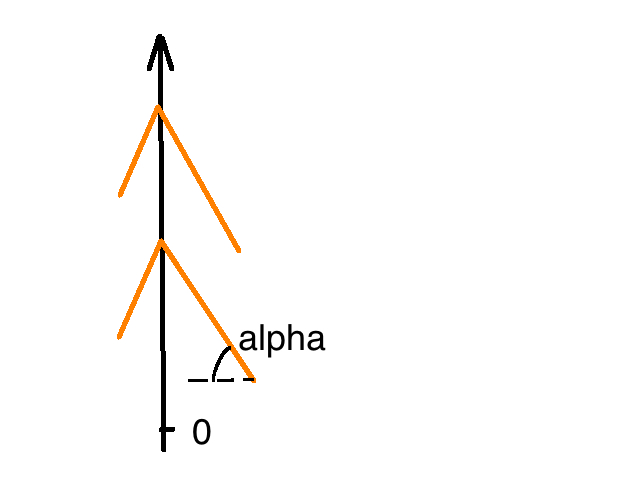
\includegraphics[height = 100pt]{6.png}	
\end{center}
Зафиксировав угол $\alpha$, единица однозначно задается координатой на $\mathbb{R}$, отсюда мощность всех таких единиц будет континум. 
\\ \\ \\

 
\noindent \textbf{Задача7.} 
\textit{Нет, нельзя} \\
\textit{Решение:}\\
Нет, нельзя. Будем решать методом от противного.\\
Для начала сопоставим каждой восьмерке 2 ее рациональные координаты, лежащие в разных полушариях этой восьмерки. Такое мы всегда сможем сделать, так как как на отрезке $a$, так и на $b$ есть хотя бы одно рациональное число, а значит на их пересечение мы получаем рациональные координаты. \\
\begin{center}
	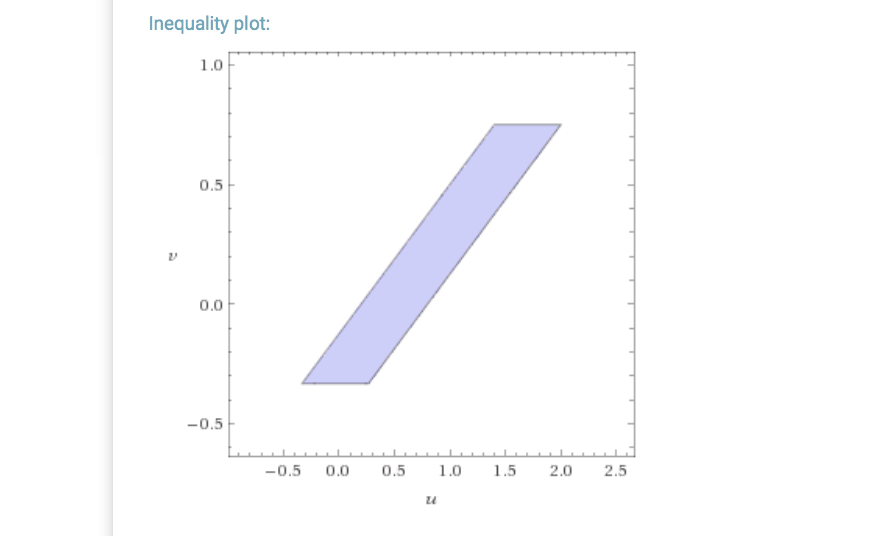
\includegraphics[height = 100pt]{7.png}	
\end{center}
Заметим, что для двух разных непересекающихся восьмерок эти два числа совпадать не могут.\\
Получившиеся пары рациональных чисел есть подмножество $\mathbb{Q}^2 \sim \mathbb{Q}$ , которое счетно $\Rightarrow$ противоречие.
\end{document}